% -----------------------------------------------------------------------
% -----------------------------------------------------------------------
% -----------------------------------------------------------------------
% Einleitung
% -----------------------------------------------------------------------
% -----------------------------------------------------------------------
% -----------------------------------------------------------------------
\chapter{Introduction}

\section{Motivation: An Open-Domain Comparative Argumentative Machine (CAM)}

tbd


\chapter{Background}
\section{Related Work}
\label{sec:argth}
\label{sec:argmine}
A general introduction on the research topic \emph{Argument Mining} is given in \cite{Lippi2016Argumentation-M}.
 The authors introduced five dimensions to describe argument mining problems: granularity of input, the genre of input, argument model, the granularity of target and goal of analysis.  Furthermore, the typical steps of argument mining systems are described. First, the input must be divided into argumentative (e.g. claim and premise) and non-argumentative parts. This step is described as a classification problem. Second, the boundaries of the argumentative units must be identified; this is understood as a segmentation problem. Third, the relations between argumentative units must be identified. For instance, claims and premises might be connected with a \emph{support} or a \emph{attack} relation.


%07 biomed


A system which is capable of recognising comparative sentences and their components such as the compared entities, the property which is used to compare the entities and the direction of comparison was presented in \cite{fiszman2007interpreting}. The evaluation showed that the outcome has a high quality (f1 score of 0.81). However, the presented system is specific to the domain of studies on drug therapy. The system used patterns generated from hand-selected sentences, as well as domain knowledge. Therefore, the methods cannot easily be transferred for the problem of this thesis.

%  12 sci
% TODO 13. April: Beispiel für Syntaktische Features
In \cite{park2012identifying}, the authors presented another domain-specific approach on argumentative sentence detection. The problem is formulated as a binary classification task (a sentence is either comparative or not). As in \cite{fiszman2007interpreting}, the features are tailored for medical publications. Features to capture the presence of specific words are used, many of them bound to the medical domain. The analysis of 274 sentences resulted in syntactic features. Similar to \cite{fiszman2007interpreting}, the features cannot be directly transferred to other domains.

% 10 biomed
A recent publication on \emph{Comparative Argument Mining} is \cite{gupta2017identifying}, where a set of rules for the identification of comparative sentences (and the compared entities) is derived from \emph{Syntactic Parse Trees}. With those rules, the authors achieved a f1 score of 0.87 for the identification of comparative sentences. The rules were obtained from 50 abstracts of biomedical papers. Such being the case, they are domain dependent.\newline

The challenges occurring while processing texts from social media are described in \cite{Snajder2017Social-Media-Ar}.  In this publication, social media is broadly defined as \enquote{less controlled communication environments [...]}. Besides the noisiness of text, missing argument structures and poorly formulated claims are mentioned. It is expected that the text used in this thesis will have the same shortcomings. Additionally, \cite{Snajder2017Social-Media-Ar} emphasized that analyzing social media texts can delivery reasons behind opinions.

In addition to the challenges mentioned above, \cite{Dusmanu2017Argument-Mining} also points to the specialized jargon in user-generated content like hashtags and emoticons. With this in mind, \cite{Dusmanu2017Argument-Mining} classified tweets about the \enquote{Brexit} and \enquote{Grexit} either as argumentative or as non-argumentative. Besides features used in other mentioned papers, new features covering hashtags and sentiment are added. They achieved a f1 score of 0.78 (using Logistic Regression) for the classification. It must to be said that the data set is small (1887 tweets) and the domain is rather specific.\newline

Publications dealing with the identification of argument structures are of relevance for this thesis, as they provide valuable insights on the suitability of features and algorithms.

%what works and what does not
In \cite{Aker2017What-works-and-}, the authors summarized and compared features used in other publications for identification of argumentative sentences. In addition to the algorithms used in the publications, a Convolutional Neural Network (as described in \cite{Kim2014Convolutional-N}) was tested. Two existing corpora and six different classification algorithms were used. The comparison resulted in the insight that structural features and Random Forests worked the best.

A two-step procedure to identify components of arguments (such as claim and premise) and their relationships (like \enquote{premise A supports claim B}) is presented in \cite{Stab2014Identifying-Arg}. The identification step is formulated as a multi-class classification. For the identification of argumentative components, a f1 score of 0.72 is reported.

%essence of a claim
How different datasets represent the argumentative unit of a \emph{claim} is analysed in \cite{Daxenberger2017What-is-the-Ess}. After an analysis of the data sets and their annotation scheme, the authors conducted two experiments.
In the first one, each learner was trained and evaluated (10-fold cross-validation) on each dataset one after another. On average, the macro f1 score for identifying claims was 0.67 (all results ranging from 0.60 to 0.80). No significant difference between the results of Logistic Regression the neural networks was found. In isolation, lexical features, syntactical features and word embeddings were most helpful. Structural features turned out to be the weakest.
The second experiment was conducted in a cross-domain fashion. For each pair of datasets, one was used as the training set and the other one as the test set. The average macro f1 score was 0.54. In this scenario, the best feature combination outperformed all neural models. However, it is assumed that there might not be enough training data for the neural models.
As the last point, the authors noted that all claims share at least some lexical clues.


The role of discourse markers in the identification of claims and premises are discussed in \cite{Eckle-Kohler2015On-the-Role-of-}. A discourse marker is a word or a phrase which connects discourse units. For instance, the word \enquote{as} can show a relation between claim and premise: \enquote{As the students get frustrated, their performance generally does not improve}.  A similar function for words like \enquote{better}, \enquote{worse} or \enquote{because} is expected in this thesis. The authors showed that discourse markers are good at discriminating claim and premises. If claim and premise are merged into one class \enquote{argumentative}, this can be used to identify argumentative sentences. The f1 score is not presented, but the accuracy is between 64.53 and 72.79 percent.



\section{Domain-Specific Comparative Systems}
Many comparison portals can be found on the internet. It is not unusual to see a television commercial those comparison portals, which suggest that they are used frequently every day.

Most portals are specific to a few domains and a subset of properties, for example, car insurances and their price. Because of that, the portals have restrictions. Comparisons are only possible between objects of the domains and predefined properties. Source of the data is usually databases. Humans are involved in gathering, entering and processing the data.

Comparison Portals solely compare and deliver facts. Because of that, they can only hint to choose X over Y based on the facts collected.  However, an insurance X might be the best in the comparison (e.g. best price), while the internet is full of complaints about lousy service.

Examples of Comparative Portals are \emph{Check24.de\footnote{\url{https://check24.de} (checked: 13.04.2018)}, Verivox.de\footnote{\url{https://verivox.de} (checked: 13.04.2018)}, Idealo.de\footnote{\url{https://idealo.de} (checked: 13.04.2018)}, GoCompare.com\footnote{\url{https://gocompare.com} (checked: 13.04.2018)},} and \emph{Compare.com}\footnote{\url{https://compare.com} (checked: 13.04.2018)} just to name a few.

As an example, Check24.de can compare a wide variety of different objects like several insurances, credit cards, energy providers, internet providers, flights, hotels and car tires. After the user entered some details (based on the object type, Check24 shows a ranking of different providers. The user can choose different properties to re-rank the list.
For instance, to compare different DSL providers, the user has to enter her address (figure  \ref{img:check24_1}), how fast the internet should be and if she wants telephone and television as well. She can then select price, speed, and grade (rating) to sort the resulting list (figure figure \ref{img:check24_2}).
\begin{figure}[tbp]
 \centering
	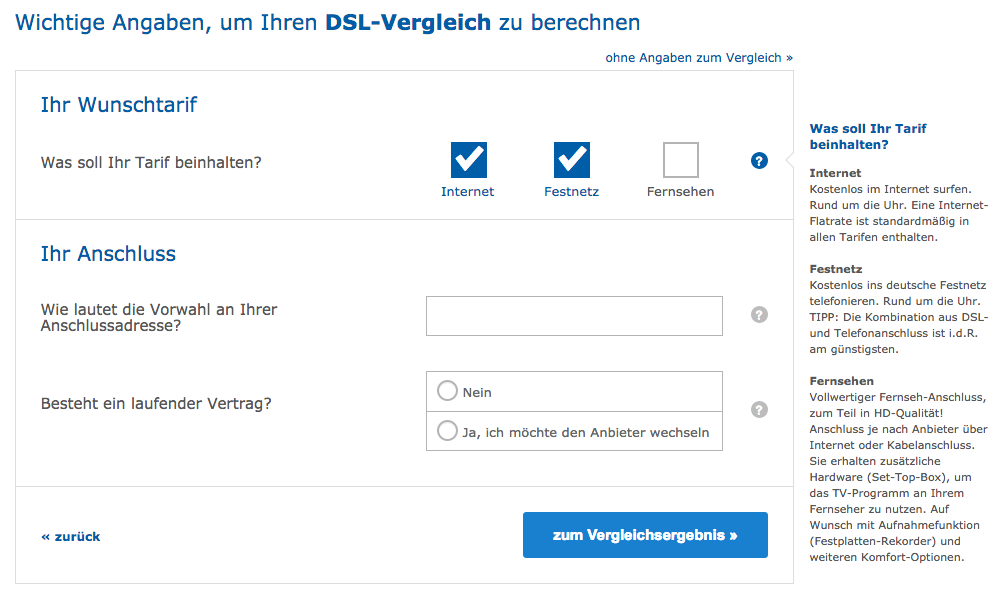
\includegraphics[width=0.8\textwidth]{images/ds-sys/check24_1}
	\caption{Check24.de asks for some data before the comparison of DSL contracts}
		\label{img:check24_1}
\end{figure}

\begin{figure}[tbp]
 \centering
	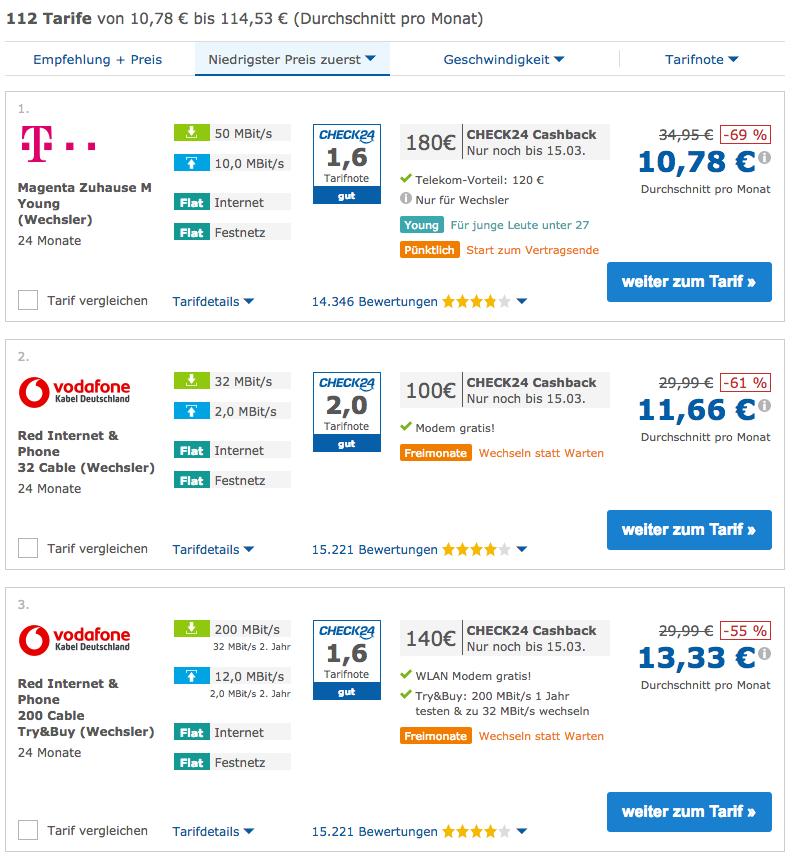
\includegraphics[width=0.8\textwidth]{images/ds-sys/check24_2}
	\caption{Check24.de DSL contract comparison result. The contracts can be sorted by domain-specific criterias.}
	\label{img:check24_2}
\end{figure}
The other sites work similar. All in all, they provide more of a ranking than a comparison.


Another interesting type of websites are Question Answering Portals like \emph{Quora.com}\footnote{\url{https://quora.com} (checked: 13.04.2018)} or \emph{GuteFrage.net}\footnote{\url{https://gutefrage.net} (checked: 13.04.2018)}. Although comparisons are not their primary goal, a lot of comparative questions are present on those sites.
On Quora, more than 2.380.000 questions have the phrase \enquote{better than} in their title. If \emph{Ruby} and \emph{Python} are added, 10.100 questions remain.\footnote{Checked via Google on 11.12.2017. Search phrase: \texttt{"better than" site:quora.com} and \texttt{ruby python "better than" site:quora.com}}
Same is true for the German site GuteFrage, though, the numbers are smaller than on Quora.\footnote{334.000 for \texttt{"besser als" site:gutefrage.net} and 78 for \texttt{ruby python "Besser als" site:gutefrage.net}}\newline

More interestingly are systems which can compare any objects on arbitrary properties, like \emph{Diffen.com}\footnote{\url{https://diffen.com} (checked: 13.04.2018)} and \emph{Versus.com}\footnote{\url{https://versus.com} (checked: 13.04.2018)}.

Versus aggregates freely available data sources like Wikipedia or official statistic reports. For example, the comparison of \enquote{Hamburg vs. Berlin} uses Wikipedia for the number of universities, worldstadiums.com for the availability of sport facilities and the Economist for the Big Mac Index. Presumably, some human processing is involved as the possible comparisons are limited. For instance, a comparison of Hamburg and Darmstadt is not possible as Darmstadt is not available on Versus. Likewise, \enquote{Ruby vs. Python} is not possible, Versus suggests to compare \enquote{Rome vs. Pyongyang} instead. Although Versus shows how many users \enquote{liked} the objects, it does not give a clear statement which one is better. For instance, it is not possible to check automatically whether Hamburg or Berlin is better for a short city trip. The user must search manually all valid properties like the number of museums, theaters, the price of public transport tickets and so on.

Similar to Versus.com, Diffen.cim aggregates different data sources (see figures \ref{img:diffen} and \ref{img:versus}). All in all, the aggregated information is similar to Versus. The comparison is also tabular. Besides the automatically aggregated data, users can add information on their own. Diffen does not enforce any restrictions on the objects of comparison, but it faces the same problem as Versus as objects are missing. A comparison between Darmstadt and Hamburg is likewise not possible: all cells for Darmstadt in the table are just empty.

\begin{figure}[htp]
 \centering
	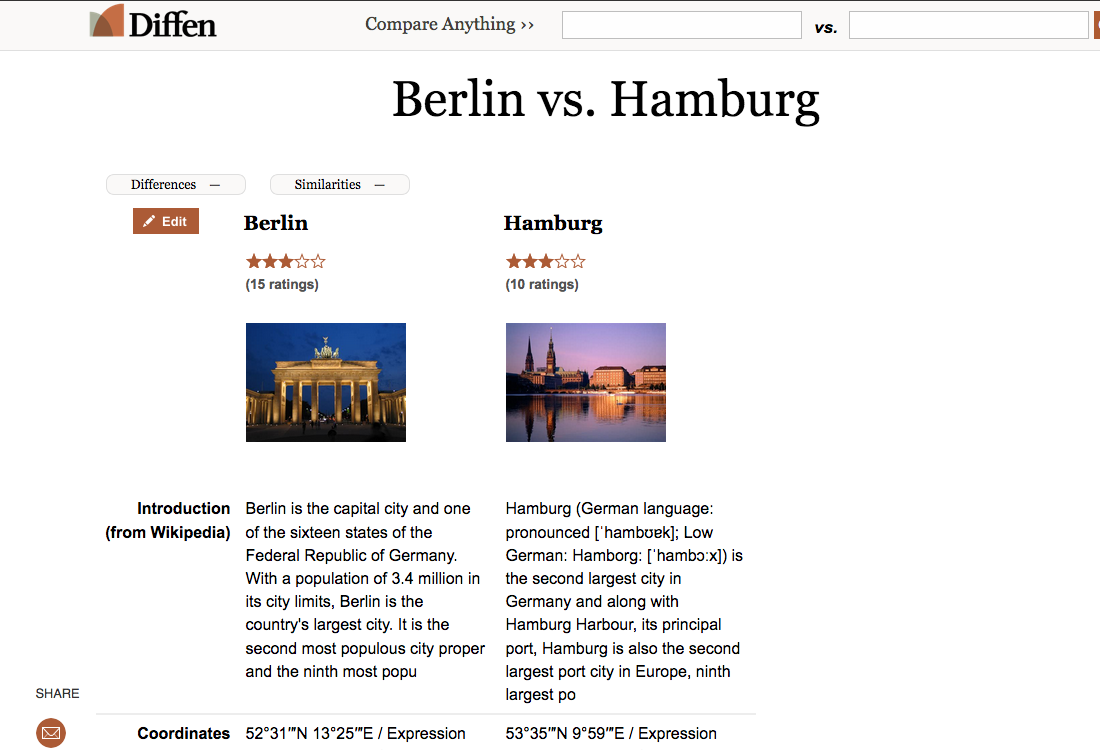
\includegraphics[width=0.8\textwidth]{images/ds-sys/diffen}
	\caption{The comparison of \enquote{Hamburg vs. Berlin} on Diffen.com}
		\label{img:diffen}
\end{figure}

\begin{figure}[htp]
    \centering
	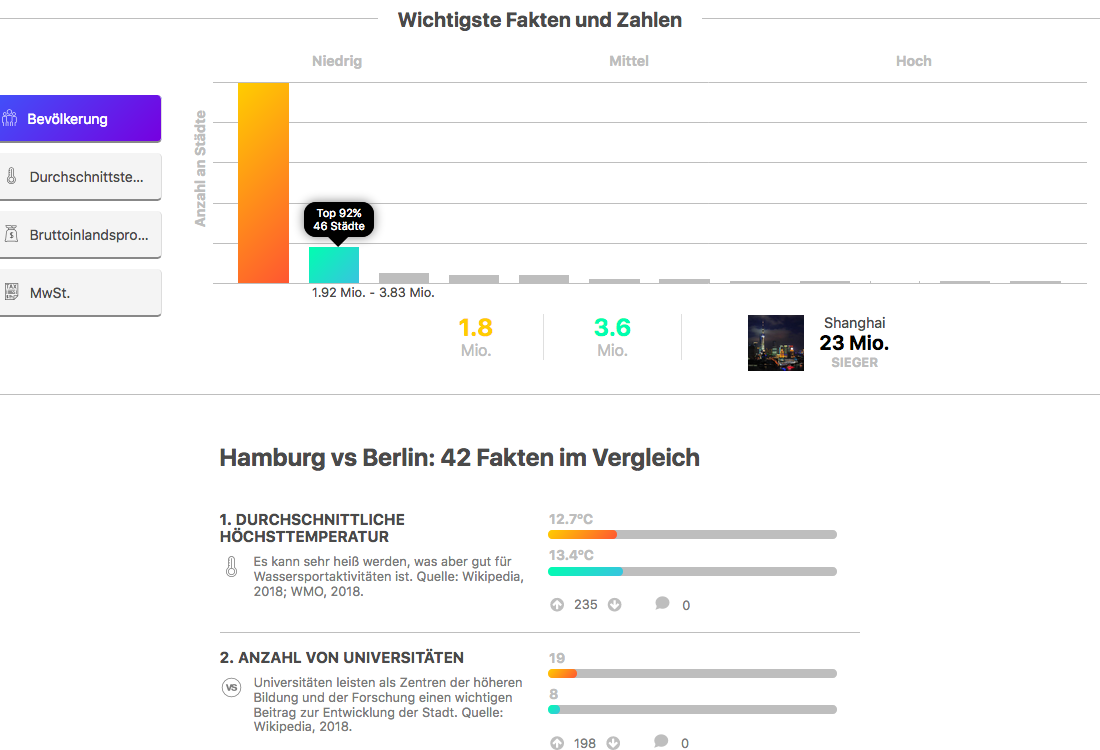
\includegraphics[width=0.8\textwidth]{images/ds-sys/versus}
	\caption{The comparison of \enquote{Hamburg vs. Berlin} on Versus.com}
		\label{img:versus}
\end{figure}

Neither Versus nor Diffen provides a comprehensible reason why an object is better than another one. They merely aggregate facts and bring them face to face. Despite the aggregation approach of both systems, many meaningful comparisons are not possible or not helpful (like \enquote{Hamburg vs. Darmstadt}, \enquote{Java vs. C\#}, \enquote{Dr Pepper vs. Orange Juice}).
Also, the user can not define the properties for the comparison. The sites provide every information available for the objects. For instance, Versus shows 42 properties for \enquote{Hamburg vs. Berlin} and only 35 for \enquote{Hamburg vs. Munich}.
\newline

To summarize, a lot of different comparison portals exist and are widely used. Especially the domain-specific portals do a good job, but inflexibility dearly buys the performance. First, the portals can only compare objects on predefined properties. Second, the data acquisition is not fully automatic. Domain-unspecific systems are good at aggregating information but do not provide a reasonable explanation to prefer X over Y.

Adding information like comments and product reviews can enrich the comparison with reasons and opinions, such as \enquote{Ruby is easier to learn than C} or \enquote{Python is more suitable for scientific applications than Erlang as many libraries exist}.

\FloatBarrier

\section{Vector Representations for Documents}
% cosine similarity
Many machine learning algorithms work with numeric values as input. Several methods are known to transform text into numeric feature vectors.
\subsection{Bag-of-words and bag-of-ngrams}
The \emph{bag-of-words} model is a simple vector representation for documents. All words in the corpus are collected into a vocabulary $\mathcal{V}$. A document j is then representend by a vector $\vec{d_j}$ of size $|\mathcal{V}|$, where $\vec{d}_{j,i}$ is the frequency of word $\mathcal{V}_i$ in the document (the \emph{term frequency} $\text{tf}(i,j)$).

The model is fast to calculate but does not take any sequence or grammar information into accoun. It also ignores the significance of words. For instance, \enquote{\emph{the}} appears in almost every English text, while \emph{\enquote{psychology}} is seldom. Yet, this is not reflected in $\vec{d_j}$, as \enquote{\emph{the}} will get at least the same value as \emph{\enquote{psychology}}. Another problem is that the vectors are as long as the vocabulary (typically thousands of words) and sparse, which adds more parameters to learn.

The first problem can be reduced by using n-grams (hence, \emph{bag-of-ngrams}) instead of words. The vocabulary $\mathcal{V}$ will then contain all sequences n consecutive words appearing in the corpus instead of single words. In this way, some sequence information is kept. The second problem can be solved by removing all very frequent words like \emph{\enquote{the}} or \emph{\enquote{can}} (often called stopwords) and using a weighting function for the remaining words, most commonly \emph{term frequency, inverse document-frequency (tf-idf)}. With tf-idf, $\vec{d_{j,i}}$ is calculated as:

\[\vec{d_{j,i}} = \text{tf}_{i,j} \times \log{ \frac{N}{n_i} } \]

where \emph{N} is the total number of documents and $n_i$ is the number of documents the word (or n-gram) i appears in.

The other problems, sparsity and length, remain. They are solved in other vector representations.


\subsection{Mean Word Embeddings}
Word Embeddings are dense, low-dimension vector representations of words. They can be learned with neural networks. The basic idea is to train an neural network on a suitable task. They weight matrix (\emph{embedding matrix}) of a defined hidden layer then contains the word embeddings.

The matrix has the size of \mbox{$(\text{number of words in } \mathcal{V} \times\allowbreak \text{number of neurons }\allowbreak \text{in the hidden layer})$} and is initialized with random values. After the network was trained, each column represents one word in $\mathcal{V}$ and each embedding has as many components as the hidden layer has neurons. This leads to word vectors which are much smaller than $|\mathcal{V}|$.

A method to learn word embeddings using a feed-forward neural network was presented in \cite{bengio2003neural}. The network was trained to predict the most likely next word given a number of preceding context words. This exploits the \emph{distributational hypothesis} (\cite{harris1954distributional}) which states that words which appear in similar contexts have a similar meaning. For instance, the network will see that the context \enquote{\emph{feed the}} is often followed by words like \enquote{\emph{cat}} or \enquote{\emph{dog}}, but never by \enquote{\emph{chair}}. In the end, the cosine similarity\footnote{a similarity metric for vectors: $\times$} between the learned vectors of related words (like cat and dog) is much higher than the cosine similarity between unrelated words (like cat and chair).

Two popular methods to learn word embeddings (extending the basic idea) are \emph{word2vec} (\cite{NIPS2013_5021}) and \emph{GloVe} (\cite{pennington2014glove}). In this thesis, \emph{GloVe} vectors are used, were each word is represented by a vector of 300 components.

The word embeddings can be used to create a dense, low-dimension vector representation for a document. This is done by taking the average of all word vectors in the document. In doing so, each sentence is represented by a \enquote{centroid word}. The efficiency of this method for several tasks is presented in \cite{Wieting:2015aa}.

\subsection{Sentence Embeddings and InferSent}
Bag-of-words an averaged word embeddings lose sequence information. However, the sequence of words in a sentence is important for the meaning. For example, the sentence \enquote{\emph{I like cats, not dogs}} has a different meaning than \enquote{\emph{I like dogs, not cats}}, but both sentences will get the same bag-of-words vector and mean  word embedding.

Sentence embeddings aim to learn embeddings for pieces of text instead of single words. In this way, sequence information is taken into account. Several methods have been proposed to create sentence embeddings (e.g. FastSent \cite{hill2016learning} and SkipTought \cite{NIPS2015_5950}). In this thesis, \emph{InferSent} as presented in \cite{Conneau:2017aa} is used.


InferSent tries to learn sentence embedding in a similar way as word embeddings are learned. A neural network is trained on the \emph{Stanford Natural Language Inference (SNLI)} data set (\cite{snli:emnlp2015}). SNLI contains 570000 English sentence pairs. Each pair is labelled as \emph{entailment}, \emph{contradiction} or \emph{neutral}. Some examples are presented in table \ref{tbl:snli}. The authors assume that the \enquote{semantic nature} %zitat
makes the data set suitable for learning universal sentence embeddings.

\begin{table}[ht]
\caption{Example sentences from the \emph{Stanford Natural Language Inference (SNLI)} data set}
\label{tbl:snli}
\begin{tabularx}{\linewidth}{XXr}
\toprule
Premise & Hypothesis & Label \\ \midrule
A soccer game with multiple males playing. & Some men are playing a sport. & Entailment \\
A man inspects the uniform of a figure in some East Asian country. & The man is sleeping & Contradiction \\
A smiling costumed woman is holding an umbrella. & A happy woman in a fairy costume holds an umbrella. & Neutral \\
\bottomrule
\end{tabularx}
\end{table}


\begin{figure}[ht]
\centering
	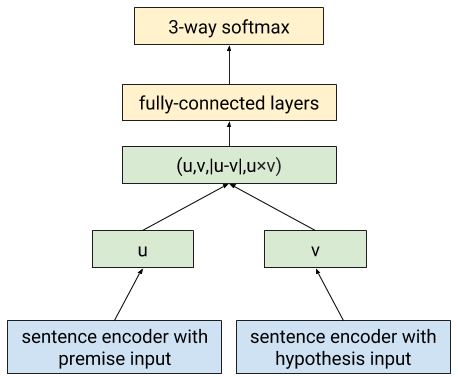
\includegraphics[width=0.5\textwidth,scale=0.5]{images/nli}
	\caption{Generic training scheme of \emph{InferSent}. Six \emph{sentence encoder} variants were tested.  (Adapted from \cite{Conneau:2017aa})}
		\label{fig:infersent}
\end{figure}


The architecture of the neural network is presented in figure \ref{fig:infersent}. Two separate encoders are used to encode the text and the hypothesis. The embeddings \emph{u} and \emph{v} are combined into a feature vector which contains the concatenation, the element-wise product and the element-wise difference of \emph{u} and \emph{v}. This vector, containing information from both sentences, is then fed into a fully connected layer and a softmax layer which outputs the probabilities of each label.

The authors tested six architectures for the sentence encoder: LSTM (\cite{hochreiter1997long}), GRU (\cite{cho2014properties}), BiLSTM with mean/max pooling (\cite{collobert2008unified}), self-attentive networks (\cite{liu2016learning}, \cite{lin2017structured}) and hierarchical ConvNet (\cite{zhao2015self}). 

Twelve transfer task\footnote{For example: binary classification (sentiment analysis, product reviews, subjectivity/objectivity, opinion polarity), multi-class classification (question type), entailment and semantic relatedness, semantic tectual similarity, paraphrase detection and caption-image retrieval.} were used to test the quality of the embeddings. For each task and encoder architecture, the embeddings were used as features. Logistic Regression was used as the machine learning algorithm.

The embeddings generated by the BiLSTM with max pooling and an embedding size of 4096 yielded the best accuracy for SNLI and the transfer tasks. Also, the embeddings were better than other state-of-the-art sentence embeddings like SkipThought.

A pretrained model for InferSent is available on GitHub\footnote{\url{https://github.com/facebookresearch/InferSent}}.

\section{HypeNet and LexNet}
\label{sec:lexnet}
HypeNet, presented in \cite{DBLP:conf/acl/ShwartzGD16}, is a method to detect hypernym relations between words. It combines distributational and dependency path based methods to create a vector representation for word pairs. LexNet, presented in \cite{DBLP:journals/corr/ShwartzD16}, is a generalisation of HypeNet, which is able to detect multiple semantic relationships between two words.

The dependency paths add information about joint occurences of the two words, while the distributational methods add information about the terms in separate contexts. Word Embeddings are used as distributational features.

For each term pair, all dependency paths were extracted. Each edge was represented as \texttt{lemma/POS/dependency label/direction}. An example is given in figure \ref{fig:hypenet}. 

\begin{figure}[h]
\centering
\caption{Dependency parse of the example sentence \emph{parrot is a bird}, where the relationship between parrot and bird is of interest. This path is represented as \texttt{X/NOUN/nsubj/< be/VERB/ROOT/- Y/NOUN/attr/>} (Adapted from \cite{DBLP:conf/acl/ShwartzGD16}).}
\label{fig:hypenet}
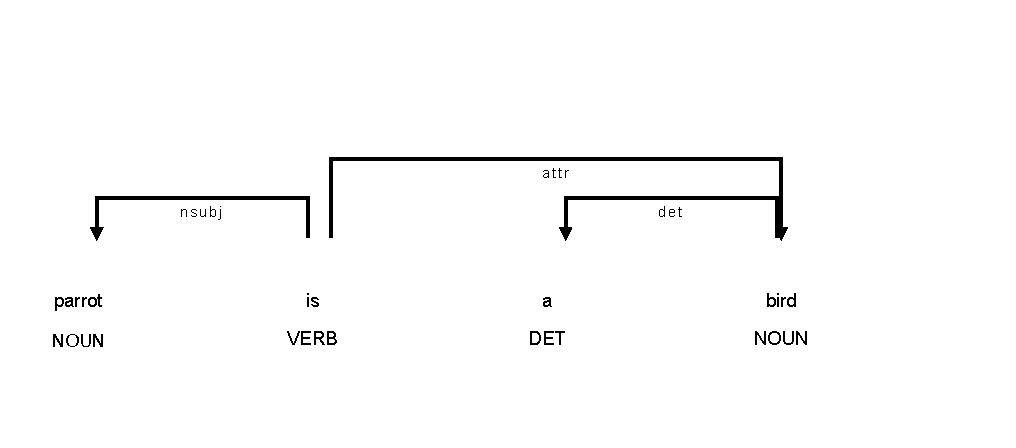
\includegraphics{images/hypenet_example}
\end{figure}


The paths were encoded using an LSTM. The average of all encoded paths was then used as the path information for the word pair. The combination of distributational and path information outperformed state-of-the-art techniques\footnote{the best compared technique (concatenation of the word embeddings) achieved an f1 score of 0.63} ( for hypernym detection, yiedling and f1 score of 0.70.\newline

The task at hand is different from the detection of semantic relations. The relation of two nouns\footnote{The situation might be different if proper nouns are also used. Fruit is an hypernym for apple, but not for the company Apple.} with respect to hypernymy is unambigous. Bird is a hypernym for parrot in all cases. Yet the task is not to search for hypernyms or any other semantic relation. It is not possible to assign the correct class by only looking at the objects. For example, there might be sentences saying that \emph{Python} is better than \emph{Ruby}, while others say it is not.

However, it is expected that the dependency path between the objects of interest adds valuable information. This thesis reuses the idea on how to extract and encode paths between two words.
\section{Gradient Boosting}
tdb